\chapter{Impacto del trabajo} \label{chp:impacto}

En este capítulo se hace un análisis del impacto general del trabajo 
desarrollado en este TFG, así como el impacto del mismo conforme a los 
Objetivos de Desarrollo Sostenible.

%%%%%%%%%%%%%%%%%%%%%%%%%%%%%%%%%%%%%%%%%%%%%%%%%%%%%%%%%%%%%%%%%%%%%%%%%%%%%%%%
%%%%%%%%%%%%%%%%%%%%%%%%%%%%%%%%%%%%%%%%%%%%%%%%%%%%%%%%%%%%%%%%%%%%%%%%%%%%%%%%

\section{Impacto general} \label{sct:impacto_impactogeneral}

Los sistemas distribuidos publicador/subscriptor se encuentran en una etapa de
grandes avances y desarrollos, pues son una tecnología ampliamente usada al 
vivir en un mundo cada día más digitalizado. 

De igual forma, la computación en la nube ha sufrido grandes avances, al 
proporcionar una plataforma en la que los usuarios pueden desplegar sus sistemas
y pagar solo por los recursos usados, a diferencia de la tradicional forma de 
desplegar sistemas de cara al público mediante tener recursos de computación 
estáticos, los cuales puedes estar desaprovechados y conllevan mayores costes.

Mediante el uso de computación en la nube y aplicando un buen sistema de 
auto-escalado, estos sistemas publicador/subscriptor proporcionarán un servicio
eficiente minimizando el coste de despliegue y mantenimiento.

En este proyecto, desde su inicio con la implementación del sistema
SilboPS\cite{thesis:tesisSVavassori} y siguiendo con la posterior mejora de 
este, que ha resultado en el sistema 
E-SilboPS\cite{tfm:victor2017}\cite{thesis:tesisVictor}, se ha desarrollado 
un sistema publicador/subscriptor que implemente, de forma óptima 
y eficiente, la función de auto-escalado, de forma que el sistema requiera
de mínima supervisión y cumpla con lo previamente mencionado.

Mediante el desarrollo de este proyecto se pretende contribuir al avance y 
mejora de los sistemas publicador/subscriptor por medio de auto-escalado 
eficiente, lo que lleva a proporcionar un mejor servicio a los usuarios de
estos sistemas, de forma que el tiempo de respuesta en el que reciben las
publicaciones sea mínimo, incluso en situaciones de mucho tráfico en el 
sistema, a la vez que se minimiza el uso de los recursos de computación,
reduciendo los costes y el malgasto energético al no desperdiciar dichos 
recursos.

El trabajo llevado a cabo en este TFG, que complementa el ya realizado en los 
trabajos previamente mencionados, mediante el estudio del comportamiento del
sistema frente a una situación que refleja una real, y los modelos de 
predicción, se pretende aplicar mejoras al auto-escalado de dicho sistema, 
aumentando su eficiencia. Este estudio se ha llevado a cabo sobre una
configuración básica 1-1-1, de forma que se identifique el punto de saturación
del sistemas bajo esta configuración, resultado el cual, mediante la aplicación
de modelos de predicción, permitirá la implementación de mejoras del auto-escalado.

Este trabajo ha permitido establecer las bases para el desarrollo de futuras 
mejoras del auto-escalado del sistema E-SilboPS, las cuales se podrán 
implementar en otros sistemas publicador/subscriptor del mismo tipo.

%%%%%%%%%%%%%%%%%%%%%%%%%%%%%%%%%%%%%%%%%%%%%%%%%%%%%%%%%%%%%%%%%%%%%%%%%%%%%%%%
%%%%%%%%%%%%%%%%%%%%%%%%%%%%%%%%%%%%%%%%%%%%%%%%%%%%%%%%%%%%%%%%%%%%%%%%%%%%%%%%

\section{Objetivos de Desarrollo Sostenible} \label{sct:impacto_ods}

% https://www.un.org/sustainabledevelopment/es/objetivos-de-desarrollo-sostenible/
% https://www.agenda2030.gob.es/objetivos/home.htm

El impacto de este trabajo sobre los 17 Objetivos de Desarrollo Sostenible 
aprobados en 2015 por los Estados Miembros de las Naciones Unidas como parte
de la Agenda 2030 para el Desarrollo Sostenible\cite{web:agenda2030}, que se 
pueden ver en la \autoref{fig:ods}, se alinea con
el \textbf{Objetivo 9. Industria, innovación e infraestructura},
el \textbf{Objetivo 11. Ciudades y Comunidades Sostenibles} y 
con el \textbf{Objetivo 12. Producción y Consumo Responsable}.

\begin{figure}[htpb]
    \centering
    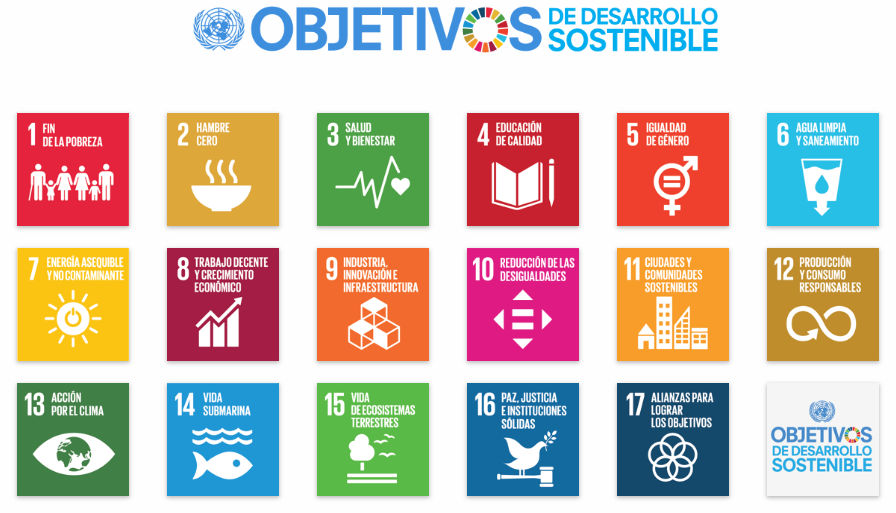
\includegraphics[width=0.75\textwidth]{images/ODS.png}
    \caption{Objetivos de Desarrollo Sostenible (\textit{ODS}). Imagen obtenida de \cite{web:agenda2030}.}
    \label{fig:ods}
\end{figure}

Los sistemas publicador/subscriptor, como el tratado en este trabajo, están 
en constante desarrollo e innovación, y son utilizados en multitud de ámbitos y
casos de uso en la vida cotidiana, por lo que sus constantes mejoras son vitales
para el funcionamiento óptimo de estos sistemas. De igual forma, estas mejoras 
conllevan un menos consumo eléctrico, al requerir de menos operaciones por cada
evento, o de desplegar un menor número de sistemas publicador/subscriptor si cada 
un puede con más carga.

A causa de esto, esta tecnología y este trabajo se alinean principalmente con el 
\textbf{Objetivo 9. Industria, innovación e infraestructura}, y de forma más 
precisa, con las metas \textbf{9.1}, al crear una infraestructura sostenible; 
\textbf{9.2} debido al constante desarrollo e innovación de la tecnología; y 
\textbf{9.4}, ya que el objetivo es modernizar los sistemas publicador/subscriptor 
y hacerlos maś eficientes.

De igual forma, se alinean, del \textbf{Objetivo 11. Ciudades y 
comunidades sostenibles}, con las metas \textbf{11.3} Urbanización inclusiva y 
sostenible, al desarrollar sistemas informáticos sostenibles 
medio-ambientalmente mediante la reducción del consumo energético de estos 
sistemas, ya sea por la mayor eficiencia de las operaciones del sistema o por
la eficiencia del sistema completo, requiriendo de menos sistemas de este tipo
al poder aumentar la carga de cada uno, requiriendo de menor número de sistemas 
desplegados.

Por último, este trabajo, al reducir el consumo energético de estos sistemas 
mediante aumentar la eficiencia, también están relacionadas con las metas del
\textbf{Objetivo 12. Producción y consumo responsables}, principalmente, con la
\textbf{12.A} Ciencia y Tecnología para Sostenibilidad, al desarrollar un sistema
que puede ser usado para impulsar la transformación digital y llevar esta 
tecnología a lugares poco digitalizados.

El impacto medioambiental del trabajo desarrollado en este TFG es mínimo, pero
una vez cumplido el objetivo último de este proyecto (maximizar la eficiencia 
del auto-escalado de los sistemas publicador/subscriptor basados en contenido
mediante E-SilboPS), si estas mejoras se implantasen de forma generalizada en 
la sociedad, junto con la constante digitalización de la vida cotidiana, 
se podría reducir la contaminación producida por estos sistemas en gran medida, 
al ser estos más eficientes.

De forma adicional, este proyecto tiene un potencial impacto en todas aquellas
áreas que se beneficiarían de una mayor sostenibilidad mediante la 
transformación digital resultante de implementar y usar este tipo de sistemas,
principalmente, en el Internet of Things y en Smart Cities.